\usetikzlibrary{calc}
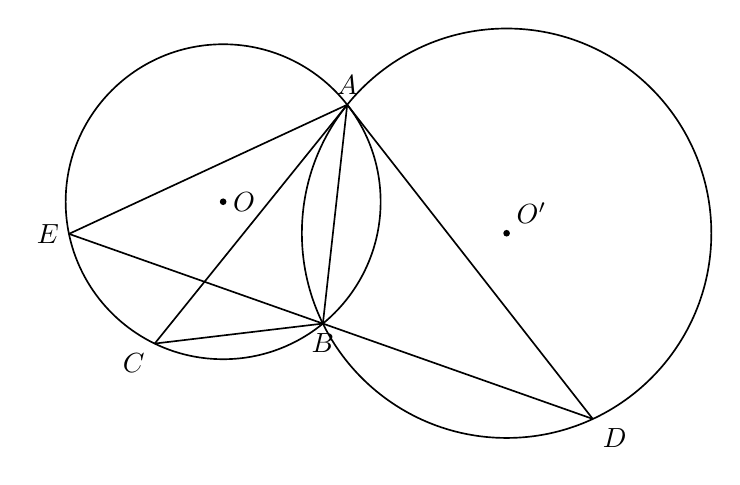
\begin{tikzpicture}[x=1cm,y=1cm,line width=.6pt,font=\normalsize]
\coordinate (O1) at (0.0000,0.0000);
\coordinate (O2) at (3.6000,-0.4000);
\coordinate (A) at (1.5757,1.2317);
\coordinate (B) at (1.2669,-1.5475);
\coordinate (C) at (-0.8690,-1.8013);
\coordinate (D) at (4.6946,-2.7584);
\coordinate (E) at (-1.9579,-0.4083);
\draw (O1) circle[radius=2.0000cm];
\draw (O2) circle[radius=2.6000cm];
\draw (A)--(B);
\draw (A)--(C);
\draw (A)--(D);
\draw (A)--(E);
\draw (C)--(B);
\draw (E)--(B);
\draw (B)--(D);
\fill (O1) circle[radius=1.2pt];
\fill (O2) circle[radius=1.2pt];
\node[above] at (A) {$A$};
\node[below] at (B) {$B$};
\node[below left] at (C) {$C$};
\node[below right] at (D) {$D$};
\node[left] at (E) {$E$};
\node[right] at (O1) {$O$};
\node[above right] at (O2) {$O'$};
\end{tikzpicture}
